\chapter{Getting started}
\thispagestyle{fancy}
\label{ch:getting-started}

\begin{action}
Start \MATLAB{} by clicking \guitext{Start} \ding{217} \guitext{Programs} \ding{217} \guitext{MATLAB} \ding{217} \guitext{MATLAB~R2009a} and click on \guitext{MATLAB~R2009a}.
\end{action}
\begin{action}
Go to \guitext{Desktop} in the menu bar and select \guitext{Desktop Layout} and then choose \guitext{Command Window Only}.
\end{action}

\noindent The Command Window\index{Command Window} is the window where you type your commands at the `\verb#>>#'-sign, also known as `prompt'\index{prompt}. These commands are then being executed by \MATLAB{} after pressing the \guitext{Enter} key.

\section{Creating your own work directory}



To create your own work directory\index{work directory}, click the \guitext{Browse for Folder} button (see Figure \ref{fig:browse-for-folder}) located to the right of the \guitext{Current Directory} drop-down list on the \MATLAB{} button bar. This button is used to change or create your work directory. Click to create your work directory or to change the directory to the directory you will be working from. Now go to the \guitext{Desktop} menu and click a checkmark next to \guitext{Current Directory}. You will see that you are now in the directory you selected through using the \guitext{Browse for Folder} button.

\begin{figure}[!htbp]
  \centering
    \fbox{
\includegraphics[width=1.0\textwidth]{./../eps/browse-for-folder}}
  \caption{Location of the ``browse for folder''-button.}\label{fig:browse-for-folder}
\end{figure}


\hintbox{Make it a habit to start every new exercise by selecting the appropriate directory for that exercise. Be sure that you are in that directory when executing your commands.}


\begin{action}
Type
\end{action}
\prompt{Groningen = 2.33}
\noindent and then press ``Enter'', keeping in mind that `{\tt \textgreater\textgreater}' is the command prompt. Note that the \MATLAB{} Command Window now displays the following output:
\begin{verbatim}
Groningen = 

    2.3300

\end{verbatim}
This output lets you know that \MATLAB{} has created a variable named \verb#Groningen# whose value is equal to \verb#2.3300#.

Go to the \guitext{Desktop} menu and click a checkmark next to \guitext{Workspace}, and you will see the \verb#Groningen# variable listed in the \MATLAB{} Workspace. Alternatively, you can type \verb#who#\index{who@\texttt{who}} or \verb#whos#\index{whos@\texttt{whos}} at the command prompt. These commands will list the variables in your Workspace in the Command Window.
\begin{action}
Type 
\end{action}
\prompt{Utrecht = 2.12}
\noindent and then press \guitext{Enter}.
\begin{action}
Type 
\end{action}
\prompt{Maastricht = 1.92}
\noindent and then press \guitext{Enter}. Both the \verb#Utrecht# and \verb#Maastricht# variables are now listed in the \MATLAB{} Workspace window.
\begin{action}
Calculate the mean of the total yearly precipitation for these three cities:
\end{action}
\prompt{Prec = (Groningen + Utrecht + Maastricht)*365/3}

\noindent Now, not only do \verb#Groningen#, \verb#Utrecht#, and \verb#Maastricht# appear in the workspace, but a new variable \verb#Prec# is also present. These short calculations are simple examples of the arithmetic operations that can be executed in \MATLAB{}. Table~\ref{tab:operations} gives an overview of the basic mathematic operators used in \MATLAB{}.
\begin{table}[t]
\caption{\MATLAB{} operations.}
\label{tab:operations}
\vspace{-0.5em}
\centering
\begin{tabular}{|l|l|l|}
\hline
\textbf{Operation}&\textbf{Symbol}&\textbf{Example}\\
\hline
Addition\index{addition}&\verb#+#&\verb#5+6.7#\\
\hline
Subtraction\index{subtraction}&\verb#-#&\verb#8.63-5.24#\\
\hline
Multiplication\index{multiplication}& \verb#*#&\verb#3*2#\\
\hline
Division\index{division}& \verb#/#&\verb#1/4#\\
\hline
Exponentiation\index{exponentiation}& \verb#^#&\verb#3^2#\\
\hline
\end{tabular}
\end{table}
Note: The square root is merely an instance of the Exponentiation notation:  \verb#A^0.5#$\equiv$\verb#sqrt(A)#\index{sqrt@\texttt{sqrt}}.

\begin{action}
Clear the workspace using the command \verb#clear#\index{clear@\texttt{clear}}
\end{action}
\begin{action}
Assign the value 1 to the variable \verb#ExampleVar#:
\end{action} 
\prompt{ExampleVar = 1}
\begin{action}
Assign the value 14 to the variable \verb#EXAMPLEVAR#:
\end{action}
\prompt{EXAMPLEVAR = 14}
\begin{action}
Check the workspace by typing:\\
\end{action}
\prompt{whos}
\noindent and then pressing the \guitext{Enter} key.
\begin{verbatim}
  Name             Size                   Bytes  Class          Attributes

  EXAMPLEVAR       1x1                        8  double array
  ExampleVar       1x1                        8  double array

\end{verbatim}
This procedure is meant to demonstrate that \MATLAB{} is case-sensitive\index{case-sensitive}: \verb#EXAMPLEVAR# and \verb#ExampleVar# are two different variables. Another way to check structures of variables entered into the \MATLAB{} Workspace is to double-click the variable in the \MATLAB{} \guitext{Workspace} window. This opens the variable up in the array editor. Check the value of the variable \verb#EXAMPLEVAR# by double-clicking its variable in the \guitext{Workspace} window.
\begin{action}
Check the value of the variable \verb#EXAMPLEVAR#.
\end{action}


\hintbox{\label{tip:naming-conventions}Be aware that as we work through the manual, the use of any special text characters (such as {\tt*}, {\tt\&}, {\tt\MVAt}, {\tt\#}, and {\tt?} ) within variable names is prohibited, the exception being the underscore `{\tt\_}' character. This is because these characters often have special effects on operations. Variable names can contain up to 31 characters, but must start with a letter followed by any combination of letters, digits or underscores.}

\begin{action}
Now, go to the \guitext{Desktop} menu and click a checkmark next to \guitext{Command History}. This opens a new window within the \MATLAB{} Graphical User Interface\index{Graphical User Interface} (GUI\index{GUI}) listing the commands that you have entered in the \guitext{Command Window}. Figure \ref{fig:gui} shows you what your GUI should look like now. 
\end{action}


\begin{figure}[!ht]
  \centering
    \fbox{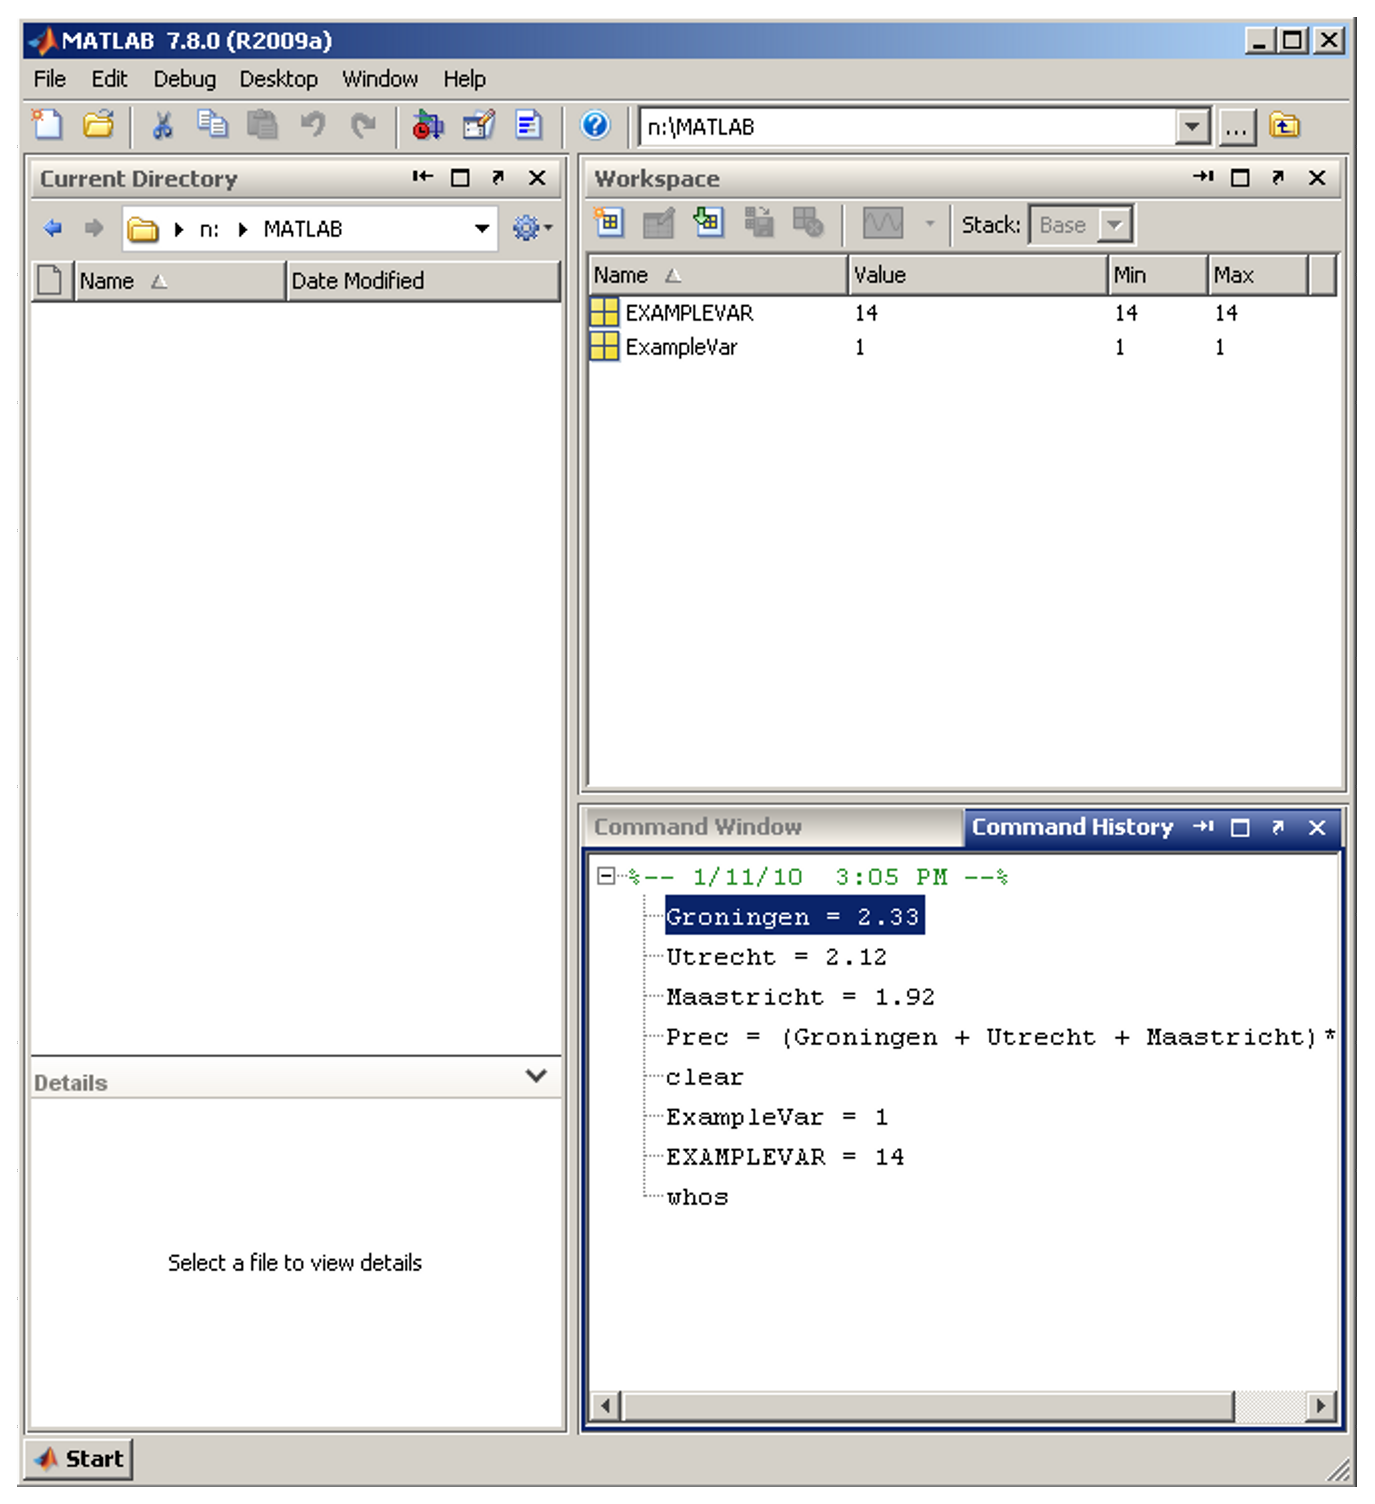
\includegraphics[width=0.9\textwidth]{./../eps/gui.eps}}
  \caption{\MATLAB{} Graphical User Interface (GUI). Note that the Command Window and Command History are docked into the same panel. You can change the layout of your GUI by clicking the title bar of the panel that you want to put somewhere else, and moving the mouse pointer while holding down the left mouse button.}\label{fig:gui}

\end{figure}


\hintbox{\MATLAB{} remembers the commands that have been typed at the prompt. You can use the up and down arrows to select any previously typed commands. You can also check the \guitext{Command History} item in the \guitext{Desktop} menu.}


